
\documentclass{article}

\usepackage[ngerman]{babel}                     %for german umlauts
\usepackage[utf8]{inputenc}
\usepackage{subfigure}
\usepackage{float}
% \usepackage[ansinew]{inputenc}        %for german umlauts

\usepackage{graphicx}
\usepackage{hyperref}

\usepackage{amssymb}    %for different fonts
\usepackage{amsmath}
% Geht nicht: \usepackage{bbm}
% \usepackage[usenames,dvips]{color} %only way to get it running with pdf:(
% \usepackage[pdftex,usenames,dvipsnames]{color}        % does not work
% \usepackage{color}
\usepackage{verbatim}
\usepackage{polynom}

\setlength{\parindent}{0pt}
\addtolength{\hoffset}{-1cm}
\addtolength{\voffset}{-1cm}
\addtolength{\textheight}{3cm}
\addtolength{\textwidth}{1cm}

\newcommand{\im}{\operatorname{Im}}
\newcommand{\rg}{\operatorname{rg}}
\newcommand{\ggt}{\operatorname{ggT}}

\begin{document}

\section*{\begin{center} Mustererkennung - Aufgabenblatt 03 \end{center}}
\begin{center}
  André Hacker und Dimitri Schachmann \\
\end{center}


\subsection*{1. Gaussverteilung}
	Zuerst die Lösung nach der neuen Definition der Aufgabe (gemäß Mail):\\
	Der Schwellenwert $S(x)$ ist eine Funktion in Abhängigkeit vom zu klassifizierenden Objekt x (hier 1-d)
	\[
	  S(x) = P(C_1|x) - P(C_2|x)
	\]
	Ist $S(x)$ positiv, ist die Wahrscheinlichkeit für Klasse $C_1$ höher und wir wählen diese.\\
	Wir formen mit Hilfe Bayes-rule um
	\begin{align*}
		S(x) &= P(C_1|x) - P(C_2|x)\\
		&= \dfrac{P(C_1 \cap x)}{P(x)} - \dfrac{P(C_2 \cap x)}{P(x)}\\
		&= \dfrac{P(C_1) P(x|C_1)}{P(x)} - \dfrac{P(C_2) P(x|C_1)}{P(x)}\\
		&= \dfrac{P(C_1) P(x|C_1) - P(C_2) P(x|C_1)}{P(x)}
	\end{align*}
	Die einzelnen Komponenten haben übrigens spezielle Bezeichnungen:
	\[
		Posterior = P(C_1|x) = \dfrac{P(C_1)P(x|C_1)}{P(x)} = \dfrac{Prior \cdot Posterior}{evidence}
	\]\\
	Da uns nur interessiert ob $S(x)$ größer oder kleiner 0 ist können wir $P(x)$ ignorieren (ist der gleiche Teiler für beide Brüche, wir können also die Gleichung mit $ P(x) $ multiplizieren). Die Wahrscheinlichkeit $P(x|C_1)$ ist nun genau durch die Dichtefunktion der Normalverteilung für $C_1$ beschrieben, so dass sich für die Klassifizierung folgende Formel ergibt
	\begin{align*}
		S'(x) &= P(C_1) P(x|C_1) - P(C_2) P(x|C_1) \\
		&= P(C_1) \cdot \dfrac{1}{\sqrt{2\pi}\sigma_1} e^{\dfrac{-(x-\mu_1)^2}{2\sigma_1^2}} - P(C_2) \cdot \dfrac{1}{\sqrt{2\pi}\sigma_2} e^{\dfrac{-(x-\mu_2)^2}{2\sigma_2^2}}
	\end{align*}

\subsection*{1. Gaussverteilung (alte Definition)}
	Nun die Lösung für die Aufgabe wie sie im Tutorium besprochen und auf dem Blatt beschrieben war (hatten wir schon fertig als die Mail kam)\\
	Gegeben 2 eindimensionale Normalverteilungen $f_1(x,\mu_1, \sigma_1)$, $f_2(x,\mu_2, \sigma_2)$ kann man den Schwellenwert für x berechnen indem man die folgende Gleichung nach x auflöst:
	\[
		f_1(x,\mu_1, \sigma_1) = f_2(x,\mu_2, \sigma_2)
	\]
	\[
		\dfrac{1}{\sqrt{2\pi}\sigma_1} e^{\dfrac{-(x-\mu_1)^2}{2\sigma_1^2}} = \dfrac{1}{\sqrt{2\pi}\sigma_2} e^{\dfrac{-(x-\mu_2)^2}{2\sigma_2^2}}
	\]
	Der Schwellenwert x ist dann der Schnittpunkt der beiden Kurven.\\
	Die Klassifizierung ist auf den ersten Blick denkbar einfach: Liegt ein Punkt $x'$ vom Schwellwert aus gesehen eher bei $\mu_1$, so gehört er zu Klasse 1, und umgekehrt.\\
	Das ist allerdings zu kurz gedacht, weil tatsächlich gibt es zwei Schnittpunkte. Z.B. gibt es nicht nur einen Schwellenwert, wenn die Verteilungen dich beieinander liegen aber sehr unterschiedliche Höhe (Varinanz) haben.\\
	
	Durch einsetzen und p-q-Formel haben wir folgendes erhalten (nicht mehr abgetippt, da nach neuer Aufgabenstellung nicht gefordert):
	\[
		x^2
		+ x\left( \frac{2(\mu_2 \sigma_1^2 - \mu_1\sigma_2^2)}{\sigma_2^2 - \sigma_1^2} \right)
		+ \left( \dfrac{\mu_1^2\sigma_2^2 - \mu_2^2\sigma_1^2-2ln(\dfrac{\sigma_2}{\sigma_1}) \sigma_1^2 \sigma_2^2}{\sigma_2^2 - \sigma_1^2} \right)
		= 0
	\]
	\[
		x = \frac{2(\mu_1\sigma_2^2 - \mu_2 \sigma_1^2)}{\sigma_2^2 - \sigma_1^2}
		\pm \sqrt{ \left( \frac{2(\mu_2 \sigma_1^2 - \mu_1\sigma_2^2)}{\sigma_2^2 - \sigma_1^2} \right)^2 - \left( \dfrac{\mu_1^2\sigma_2^2 - \mu_2^2\sigma_1^2-2ln(\dfrac{\sigma_2}{\sigma_1}) \sigma_1^2 \sigma_2^2}{\sigma_2^2 - \sigma_1^2} \right) }
	\]
	
	Zwei Spezialfälle ergeben sich: Wenn $\mu_1 = \mu_2$ gilt, gibt es keinen Schwellenwert\\
	Wenn $\sigma_1 = \sigma_2$ gilt, liegt der Schwellwert genau in der Mitte von $\mu_1$ und $\mu_2$ also $x = \dfrac{\mu_1 + \mu_2}{2}$\\
	
	Das ganze haben wir implementiert und mit dem Wert verglichen den Matlab berechnet, wenn es die Gleichung ganz oben auflöst (identisch).
	\verbatiminput{threshold.m} %a


\subsection*{2. Fisher's Diskriminante}

	Unser Algorithmus geht für jede Kombination von 2 Klassen folgendermaßen vor
	\begin{enumerate}
		\item Den Erwartungswert $\mu_1, \mu_2$ und Kovarianzmatrizen $\Sigma_1, \Sigma_2$ (16-dimensional) für beide Klassen berechnen
		\item Optimale Projektionsrichtung mittels Fisher Kriterium berechnen
		\item Daraus ergeben sich die neuen eindimensionalen Klassen, die wir mit $\mu_1, \mu_2$ und $\sigma_1, \sigma_2$ beschreiben.
		\item Ein neues Element $\vec{x}$ wird nun klassifiziert indem die Projektion gebildet wird und dann aufgrund des Schwellwertes (siehe Aufgabe 1) die Klasse gewählt wird.
	\end{enumerate}
	
	
	Folgende (symmetrische) Matrix enthält die Erfolgsraten in Prozent.
	\begin{table}[H]
	    \begin{tabular}{|l|l|l|l|l|l|l|l|l|l|l|}
	        \hline
	 & 0 & 1 & 2 & 3 & 4 & 5 & 6 & 7 & 8 & 9 \\ \hline
	0 & 0 & 88.858 & 97.937 & 96.71 & 91.334 & 93.983 & 72.818 & 98.212 & 48.069 & 53.076 \\
	1 & 88.858 & 0 & 85.44 & 88.714 & 98.214 & 61.373 & 43.286 & 50.962 & 51.143 & 68.714 \\
	2 & 97.937 & 85.44 & 0 & 99 & 65.385 & 100 & 94 & 77.61 & 94.857 & 99.857 \\
	3 & 96.71 & 88.714 & 99 & 0 & 87.714 & 71.237 & 74.405 & 46.429 & 85.268 & 50 \\
	4 & 91.334 & 98.214 & 65.385 & 87.714 & 0 & 89.27 & 81.429 & 91.484 & 63.143 & 54.286 \\
	5 & 93.983 & 61.373 & 100 & 71.237 & 89.27 & 0 & 87.034 & 78.827 & 50.82 & 54.545 \\
	6 & 72.818 & 43.286 & 94 & 74.405 & 81.429 & 87.034 & 0 & 55.714 & 86.905 & 95.536 \\
	7 & 98.212 & 50.962 & 77.61 & 46.429 & 91.484 & 78.827 & 55.714 & 0 & 85.143 & 62.143 \\
	8 & 48.069 & 51.143 & 94.857 & 85.268 & 63.143 & 50.82 & 86.905 & 85.143 & 0 & 60.714 \\
	9 & 53.076 & 68.714 & 99.857 & 50 & 54.286 & 54.545 & 95.536 & 62.143 & 60.714 & 0 \\
	        \hline
	    \end{tabular}
	\end{table}
	%Die durchschnittliche Erfolgsrate ist 68.6319\% \\
	
	Um unsere Implementierung zu testen haben wir drei einfache Einfache zweidimensionale Beispiele gewählt und die Fisher-Diskriminante berechnet und dargestellt (Linie). Dargestellt werden die Samples der beiden Klassen, die Means (Mu), sowie die Means der Projektion (Mu Projection). Hier die Ergebnisse:
	\begin{figure}[H]
	  \begin{subfigure}
	    \centering
	    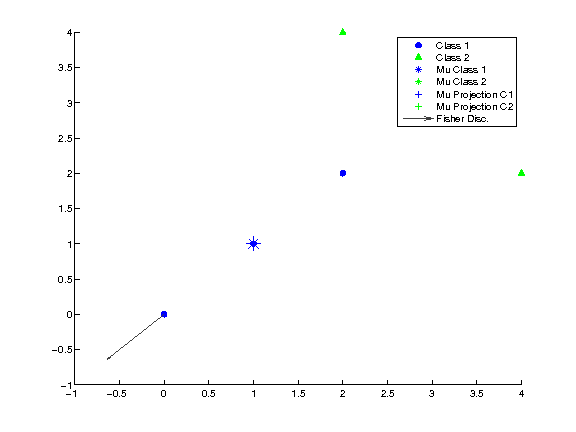
\includegraphics[scale=0.8,bb=0 0 576 432]{fisher1.png}
		\caption{Beispiel 2D Fisher Diskriminante}
	  \end{subfigure}
	\end{figure}
	\begin{figure}[H]
	  \begin{subfigure}
	    \centering
	    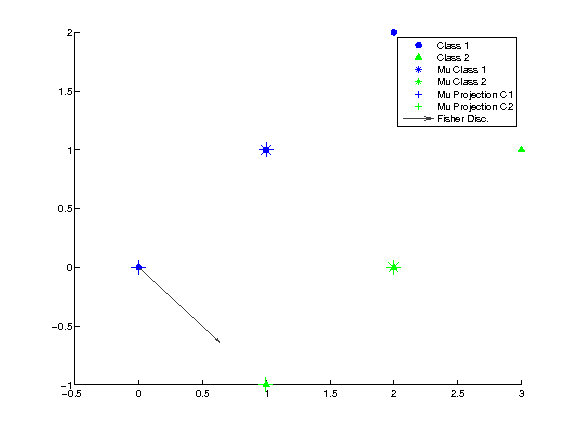
\includegraphics[scale=0.8,bb=0 0 576 432]{fisher2.png}
		\caption{Beispiel 2D Fisher Diskriminante}
	  \end{subfigure}
	\end{figure}
	\begin{figure}[H]
	  \begin{subfigure}
	    \centering
	    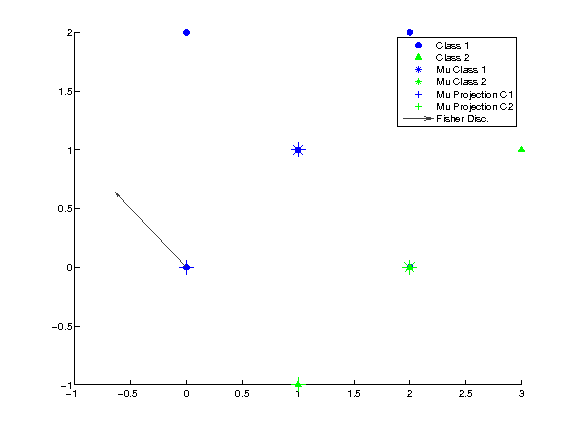
\includegraphics[scale=0.8,bb=0 0 576 432]{fisher3.png}
		\caption{Beispiel 2D Fisher Diskriminante}
	  \end{subfigure}
	\end{figure}
	
	Hier die Implementierung:
	
	\verbatiminput{fisher.m} %a


\subsection*{3. Partielle Ableitung}
	 \subsubsection*{a)}
	 	1. Plot der Funktion
		\begin{figure}[H]
		  \begin{subfigure}
		    \centering
		    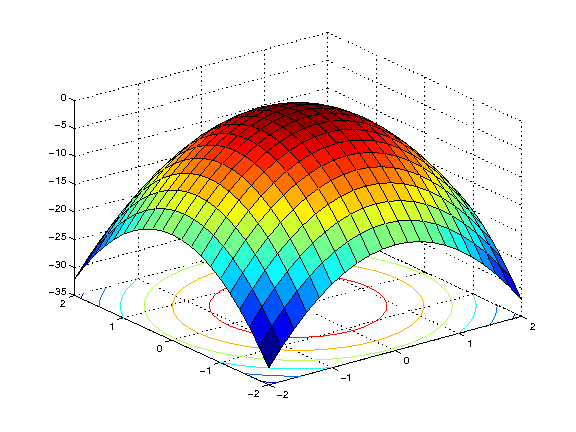
\includegraphics[scale=0.5,bb=0 0 576 432]{task3-f1.png}
			\caption{Funktionsoberfläche}
		  \end{subfigure}
		\end{figure}
	
	 	2. Partielle Ableitungen
	 	\[
	 		f(x,y) = -4 \cdot (x^2 + y^2)
	 	\]
	 	\[
	 		\dfrac{\partial f}{\partial x} = -8x
	 	\]
	 	\[
	 		\dfrac{\partial f}{\partial y} = -8y
	 	\]
	 	
	 	3. Plots der partiellen Ableitungen
		\begin{figure}[H]
		  \begin{subfigure}
		    \centering
		    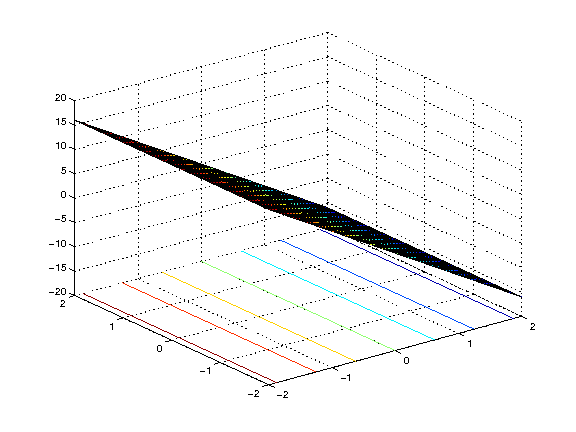
\includegraphics[scale=0.5,bb=0 0 576 432]{task3-f1-derivatedX.png}
			\caption{Partielle Ableitung nach X}
		  \end{subfigure}
		\end{figure}
		\begin{figure}[H]
		  \begin{subfigure}
		    \centering
		    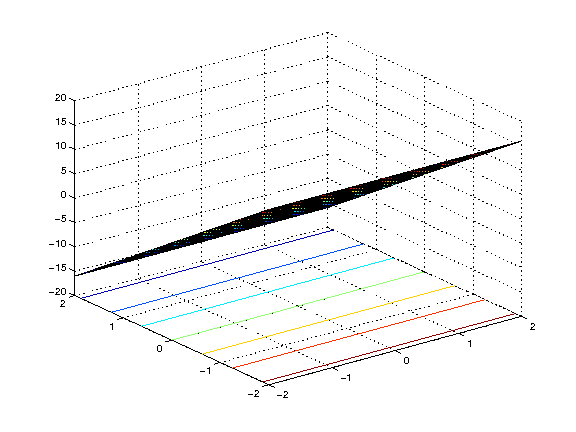
\includegraphics[scale=0.5,bb=0 0 576 432]{task3-f1-derivatedY.png}
			\caption{Partielle Ableitung nach Y}
		  \end{subfigure}
		\end{figure}
		
	 	4. Quiver Plot\\
	 	Interpretation: siehe Teil b) (analog)
		\begin{figure}[H]
		  \begin{subfigure}
		    \centering
		    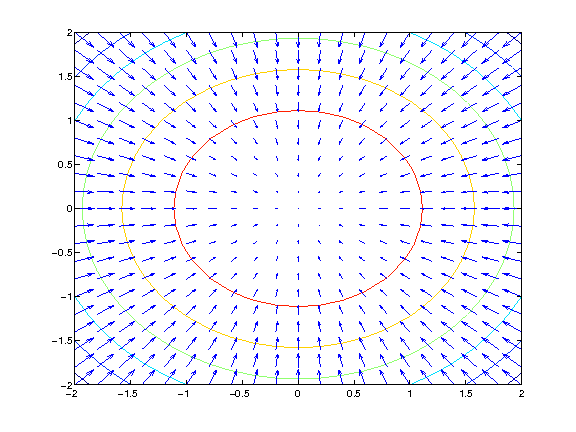
\includegraphics[scale=0.5,bb=0 0 576 432]{task3-f1-quiver.png}
			\caption{Kontur und Quiver Plot}
		  \end{subfigure}
		\end{figure}
		
		
		
		
	 \subsubsection*{b)}
	 	1. Plot der Funktion
		\begin{figure}[H]
		  \begin{subfigure}
		    \centering
		    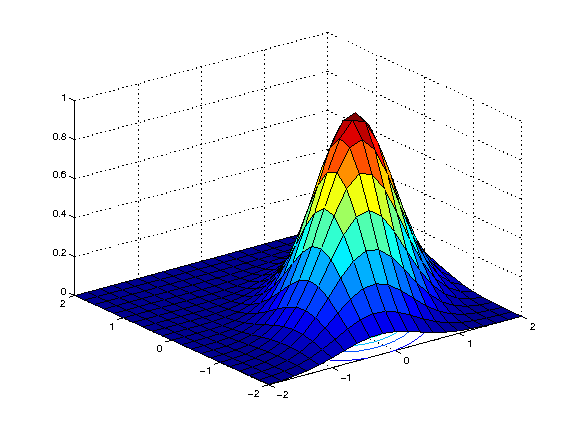
\includegraphics[scale=0.5,bb=0 0 576 432]{task3-f2.png}
			\caption{Funktionsoberfläche}
		  \end{subfigure}
		\end{figure}
	
	 	2. Partielle Ableitungen\\
	 	Wir formen zuerst die Funktion um (ausmultiplizieren), um besser ableiten zu können (Linearität ausnutzen):
	 	\begin{align*}
	 		f(x,y) &= e^{-\dfrac{(x-1/2)^2 - (x-1/2)(y+1/2) + (y+1/2)^2}{3/4}} \\
	 		&= e^{\frac{1}{3}( -4x^2 + 6x - 4y^2 - 6y + 4xy - 3 )}
	 	\end{align*}
	 	Wir haben einen Ausdruck der Form $f(g(x,y))$ mit $f=exp$, also wenden wir die Kettenregel an und leiten partiell ab.
	 	\[
	 		\dfrac{\partial f}{\partial x} = e^{\frac{1}{3}( -4x^2 + 6x - 4y^2 - 6y + 4xy - 3 )} \cdot \dfrac{1}{3} (-8x + 6 + 4y)
	 	\]
	 	\[
	 		\dfrac{\partial f}{\partial x} = e^{\frac{1}{3}( -4x^2 + 6x - 4y^2 - 6y + 4xy - 3 )} \cdot \dfrac{1}{3} (-8y - 6 + 4x)
	 	\]\\
	 	
	 	3. Plots der partiellen Ableitungen
		\begin{figure}[H]
		  \begin{subfigure}
		    \centering
		    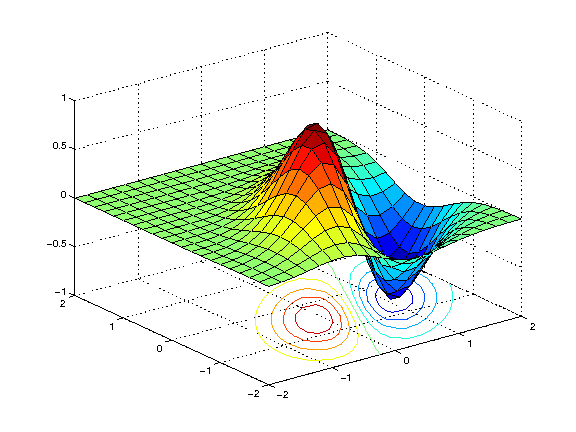
\includegraphics[scale=0.5,bb=0 0 576 432]{task3-f2-derivatedX.png}
			\caption{Partielle Ableitung nach X}
		  \end{subfigure}
		\end{figure}
		\begin{figure}[H]
		  \begin{subfigure}
		    \centering
		    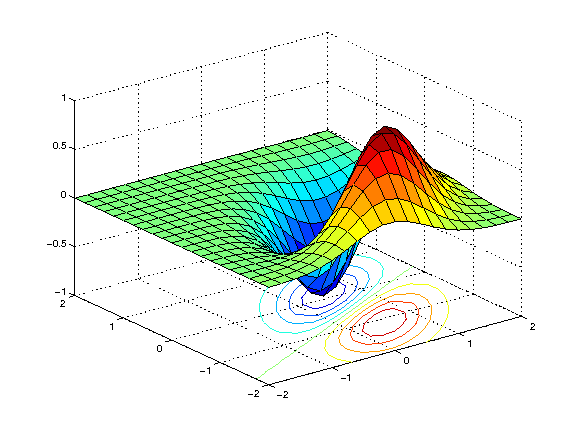
\includegraphics[scale=0.5,bb=0 0 576 432]{task3-f2-derivatedY.png}
			\caption{Partielle Ableitung nach Y}
		  \end{subfigure}
		\end{figure}
		
	 	4. Quiver Plot\\
	 	Interpretation: Die Vektoren gehen in die Richtung (bezogen auf x und y), in der die Werte der ursprünglichen Funktion am meisten steigen. Daher sind sie auch über die partiellen Ableitungen definiert, weil diese ja gerade die Steigung an der jeweiligen Stelle beschreiben (zumindest jeweils auf eine Komponente bezogen).\\
	 	Die Länge der Vektoren veranschaulicht, wie stark die Steigung an dieser Stelle ist.\\
	 	Soweit ich das verstehe entspricht das Quiver-Plot der Darstellung des sogenannten Gradienten, zumindest für ein paar ausgewählte Stellen an denen die Vektoren dann ihren Ursprung haben.
		\begin{figure}[H]
		  \begin{subfigure}
		    \centering
		    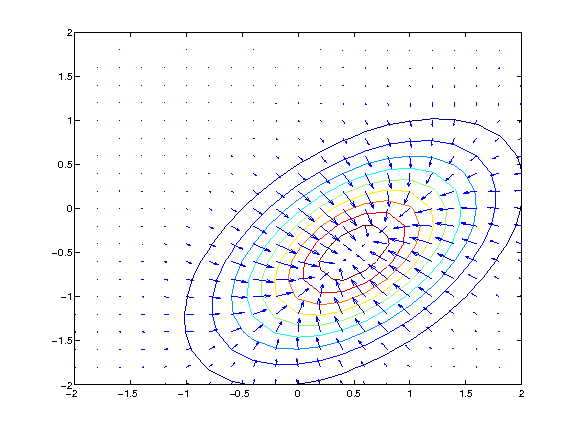
\includegraphics[scale=0.5,bb=0 0 576 432]{task3-f2-quiver.png}
			\caption{Kontur und Quiver Plot}
		  \end{subfigure}
		\end{figure}
		
		Hier der Source code:
		\verbatiminput{plotderivation.m} %a

\end{document}
